\section{Overlap Study: Further Results and Tests}
\label{app:v8}

\begin{table*}[t]
\centering\small
\setlength{\tabcolsep}{3.0pt}
\resizebox{\textwidth}{!}{\begin{tabular}{llrrrrrrrrrrr}
\toprule
 & & & \multicolumn{3}{c}{tcpBLEU} & & & \multicolumn{2}{c}{text end lag (s)} & \multicolumn{3}{c}{listener lag, completion (s)} \\
\cmidrule(lr){4-6}\cmidrule(lr){9-10}\cmidrule(lr){11-13}
Set & System & Mtgs & windows & online & speech & Omit & Ins. & p50 & p90 & 1 ch.\ p50 & per-spk p50 & per-spk p90 \\
\midrule
En$\rightarrow$Zh & \sys{}-Simul & 16 & 42.45 & 40.09 & 29.07 & 20.6 & 4.9 & 1.87 & 2.82 & 141.8 & 6.5 & 11.2 \\
 & \sys{} + LA2 & 16 & 31.41 & 34.26 & 27.49 & 25.7 & 7.0 & 2.30 & 6.09 & 255.1 & 11.0 & 104.7 \\
\midrule
Zh$\rightarrow$En & \sys{}-Simul & 16 & 23.96 & 24.53 & 16.60 & 18.6 & 6.3 & 1.94 & 2.41 & 26.0 & 7.9 & 14.9 \\
 & \sys{} + LA2 & 16 & 24.30 & 23.94 & 14.90 & 21.0 & 7.8 & 2.01 & 5.57 & 27.5 & 7.4 & 15.8 \\
\midrule
AliMeeting & \sys{}-Simul & 20 & 13.34 & 11.46 & 9.43 & 13.0 & 3.1 & 1.62 & 2.49 & 604.4 & 18.0 & 306.3 \\
 & \sys{} + LA2 & 20 & 12.41 & 11.09 & 9.14 & 15.8 & 3.6 & 2.77 & 7.91 & 734.9 & 36.7 & 194.3 \\
\bottomrule
\end{tabular}}
\caption{Whole meetings run online, all test meetings (AMI 16 per direction, AliMeeting 20; no reference boundary). tcpBLEU of the same system on the reference windows of the same meetings (windows), run online (text), and of the ASR of its synthesised speech (speech); Omit / Ins.: unscored reference units / inserted segments (\%); text end lag: last commit of a reference unit minus its end, including the delay until a window's end is detected; listener lag: end of a block's speech minus the end of its source segment, with measured computation and synthesis, on one interpreter channel (1 ch.) or one channel per speaker (Appendix~\ref{app:online7}). AliMeeting references: machine translations (Appendix~\ref{app:qe7}).}
\label{tab:online7}
\end{table*}


\paragraph{Analysis plan.} The overlap study's analysis plan (internal, not publicly registered) was fixed before any
of its test decodes; it fixes the systems, the overlap metrics and their thresholds, the causal relabelling rule, the
twelve confirmatory tests and the wording for each outcome. An amendment made before any fallback or scheduling result
fixed the short-turn fallback and the playback policies.
The speaker-blind Simul model is trained like \sys{}-Simul (same deadline-target rows, seed, 3{,}000 steps, batch 64),
from the offline speaker-blind model with the speaker tokens zeroed. Table~\ref{tab:reg8} lists the tests.

\begin{table*}[t]
\centering\small
\setlength{\tabcolsep}{4pt}
\begin{tabular}{lllrrrl}
\toprule
Test & Set & Comparison (whole meetings, online) & $\Delta$ & 95\% interval & $p_\text{Holm}$ & \\
\midrule
E-ov1-en2zh & En$\rightarrow$Zh & tcpBLEU-ov, \sys{}-Simul $-$ causal relabel & 8.54 & [3.82, 14.28] & $<$0.001 & holds \\
E-ov2-en2zh & En$\rightarrow$Zh & concurrent-speaker recall, same pair & 0.168 & [0.145, 0.194] & $<$0.001 & holds \\
E-lat-en2zh & En$\rightarrow$Zh & text lag, overlapped $-$ single ($<$0.5\,s) & -0.36 & [-0.425, -0.299] & $<$0.001 & holds \\
E-pol-en2zh & En$\rightarrow$Zh & text lag, LA2 (same model) $-$ \sys{}-Simul & 0.81 & [0.553, 1.081] & $<$0.001 & holds \\
E-ov1-zh2en & Zh$\rightarrow$En & tcpBLEU-ov, \sys{}-Simul $-$ causal relabel & 8.67 & [2.63, 12.94] & 0.002 & holds \\
E-ov2-zh2en & Zh$\rightarrow$En & concurrent-speaker recall, same pair & 0.258 & [0.219, 0.302] & $<$0.001 & holds \\
E-lat-zh2en & Zh$\rightarrow$En & text lag, overlapped $-$ single ($<$0.5\,s) & -0.21 & [-0.264, -0.167] & $<$0.001 & holds \\
E-pol-zh2en & Zh$\rightarrow$En & text lag, LA2 (same model) $-$ \sys{}-Simul & 0.23 & [0.107, 0.374] & $<$0.001 & holds \\
E-ov1-ali & AliMeeting & tcpBLEU-ov, \sys{}-Simul $-$ causal relabel & 0.63 & [-2.43, 3.51] & 0.381 & tie / fails \\
E-ov2-ali & AliMeeting & concurrent-speaker recall, same pair & 0.172 & [0.131, 0.205] & $<$0.001 & holds \\
E-lat-ali & AliMeeting & text lag, overlapped $-$ single ($<$0.5\,s) & -0.23 & [-0.325, -0.119] & $<$0.001 & holds \\
E-pol-ali & AliMeeting & text lag, LA2 (same model) $-$ \sys{}-Simul & 1.89 & [1.327, 2.496] & $<$0.001 & holds \\
\bottomrule
\end{tabular}
\caption{The twelve confirmatory tests of the overlap study, Holm-corrected together. A test holds when $p_\text{Holm}<0.05$ and
the interval excludes 0 (E-lat: lies below the 0.5\,s bound). Exact sign-flip permutation over meetings; intervals from
10,000 meeting resamples, BLEU differences with a decoder-noise draw per resample.}
\label{tab:reg8}
\end{table*}


\paragraph{All systems.} Table~\ref{tab:overlap8} gives every system on reference windows and whole meetings with the
overlap split, concurrent-speaker recall and collapse, recall of overlapped utterances under 0.5\,s and units translated
twice. \sys{}-Simul translates a unit twice more often than the offline model (\num{v8:ov:en2zh:S2dl_d1:dup} vs.\
\num{v8:ov:en2zh:O2:dup}\% in En$\rightarrow$Zh), mostly when padding puts the same words into two consecutive reads'
segments. Splitting a segment that spans two reference units in proportion to time (the default here) changes tcpBLEU by
at most a few hundredths of a point against assigning it whole to one unit.

\begin{table*}[t]
\centering\small
\setlength{\tabcolsep}{4pt}
\begin{tabular}{lrrrrrrr}
\toprule
 & \multicolumn{3}{c}{tcpBLEU$\uparrow$} & \multicolumn{2}{c}{concurrent speakers} & short & \\
\cmidrule(lr){2-4}\cmidrule(lr){5-6}
System & all & overlap & single & recall$\uparrow$ & collapse$\downarrow$ & $\le$0.5\,s$\uparrow$ & dup.$\downarrow$ \\
\midrule
\multicolumn{8}{l}{\emph{En$\rightarrow$Zh, reference windows}} \\
Cascade, same data & 36.13 & 26.21 & 41.72 & 89.3 & 9.1 & 67.8 & 1.6 \\
Cascade, turn-trained & 34.61 & 32.77 & 35.28 & 81.9 & 14.6 & 56.8 & 1.3 \\
Speaker-blind + relabel (offline) & 41.39 & 30.98 & 46.04 & 51.8 & 40.9 & 34.8 & 2.1 \\
\sys{} (offline) & 42.06 & 34.56 & 45.35 & 76.3 & 20.3 & 60.0 & 1.4 \\
\sys{} text, diarizer relabelling & 41.17 & 31.94 & 45.31 & 53.3 & 40.5 & 35.7 & 2.5 \\
\sys{} (offline) + fallback & 42.53 & 34.67 & 45.52 & 86.2 & 12.7 & 69.1 & 2.5 \\
\sys{}-Simul model + LA2 & 38.96 & 27.38 & 45.04 & 75.9 & 22.5 & 51.7 & 3.6 \\
\sys{}-Simul & 42.45 & 36.00 & 44.71 & 83.8 & 15.5 & 56.9 & 8.1 \\
\multicolumn{8}{l}{\emph{En$\rightarrow$Zh, whole meetings online}} \\
\sys{} (offline) + LA2 & 34.30 & 22.34 & 41.86 & 73.4 & 23.8 & 50.7 & 1.4 \\
\sys{}-Simul model + LA2 & 39.31 & 32.91 & 40.91 & 75.5 & 22.8 & 50.4 & 4.0 \\
\sys{}-Simul model, lag 2\,s$^\dagger$ & 40.28 & 32.24 & 43.65 & 74.4 & 24.0 & 47.8 & 6.2 \\
Speaker-blind Simul + causal relabel & 35.22 & 27.17 & 38.80 & 65.5 & 30.6 & 37.9 & 9.3 \\
\sys{}-Simul & 40.09 & 35.71 & 41.39 & 82.3 & 16.2 & 55.0 & 8.6 \\
\multicolumn{8}{l}{\emph{Zh$\rightarrow$En, reference windows}} \\
Cascade, same data & 21.96 & 14.36 & 26.31 & 87.4 & 12.0 & 67.5 & 1.0 \\
Cascade, turn-trained & 23.20 & 19.39 & 24.76 & 83.8 & 15.4 & 64.1 & 1.1 \\
Speaker-blind + relabel (offline) & 24.36 & 16.90 & 27.63 & 50.6 & 44.8 & 34.9 & 5.5 \\
\sys{} (offline) & 25.43 & 19.72 & 27.80 & 79.0 & 19.1 & 62.2 & 4.2 \\
\sys{} text, diarizer relabelling & 24.46 & 16.74 & 27.86 & 46.6 & 48.6 & 30.9 & 5.4 \\
\sys{} (offline) + fallback & 25.74 & 20.07 & 28.08 & 84.2 & 15.0 & 67.2 & 4.7 \\
\sys{}-Simul model + LA2 & 24.41 & 18.26 & 26.94 & 80.4 & 18.7 & 63.9 & 5.3 \\
\sys{}-Simul & 23.96 & 15.59 & 26.99 & 82.4 & 17.1 & 68.3 & 7.3 \\
\multicolumn{8}{l}{\emph{Zh$\rightarrow$En, whole meetings online}} \\
\sys{} (offline) + LA2 & 23.94 & 18.88 & 26.04 & 78.7 & 19.8 & 61.4 & 4.1 \\
\sys{}-Simul model + LA2 & 23.96 & 17.89 & 26.43 & 79.4 & 19.9 & 65.2 & 5.1 \\
\sys{}-Simul model, lag 2\,s$^\dagger$ & 24.69 & 19.43 & 26.80 & 76.8 & 22.3 & 66.0 & 6.7 \\
Speaker-blind Simul + causal relabel & 19.33 & 9.06 & 26.72 & 54.4 & 42.4 & 35.7 & 7.5 \\
\sys{}-Simul & 24.53 & 17.73 & 26.68 & 80.2 & 19.0 & 68.1 & 7.0 \\
\multicolumn{8}{l}{\emph{AliMeeting, reference windows}} \\
Cascade, same data & 15.70 & 9.79 & 17.96 & 93.3 & 6.5 & 60.6 & 2.1 \\
Cascade, turn-trained & 13.27 & 12.03 & 13.68 & 89.2 & 10.1 & 52.9 & 1.6 \\
Speaker-blind + relabel (offline) & 16.27 & 12.04 & 18.26 & 58.0 & 35.2 & 20.9 & 6.2 \\
\sys{} (offline) & 15.19 & 12.10 & 16.60 & 79.2 & 15.0 & 46.3 & 4.4 \\
\sys{} text, diarizer relabelling & 14.91 & 11.34 & 16.59 & 55.9 & 36.3 & 19.6 & 5.9 \\
\sys{} (offline) + fallback & 15.44 & 12.64 & 16.65 & 86.7 & 11.8 & 59.4 & 5.3 \\
\sys{}-Simul model + LA2 & 13.80 & 10.13 & 15.34 & 80.2 & 18.4 & 40.0 & 10.1 \\
\sys{}-Simul & 13.34 & 9.90 & 14.95 & 83.4 & 15.7 & 46.1 & 17.1 \\
\multicolumn{8}{l}{\emph{AliMeeting, whole meetings online}} \\
\sys{} (offline) + LA2 & 11.11 & 7.19 & 13.39 & 75.6 & 20.1 & 40.2 & 5.3 \\
\sys{}-Simul model + LA2 & 11.91 & 7.60 & 14.30 & 76.7 & 21.4 & 36.8 & 9.7 \\
\sys{}-Simul model, lag 2\,s$^\dagger$ & 12.83 & 10.17 & 14.00 & 84.8 & 13.9 & 41.2 & 17.2 \\
Speaker-blind Simul + causal relabel & 12.67 & 8.55 & 14.52 & 63.0 & 31.7 & 22.9 & 18.7 \\
\sys{}-Simul & 11.47 & 9.18 & 12.42 & 80.2 & 17.4 & 46.1 & 17.4 \\
\bottomrule
\end{tabular}
\caption{Overlap-aware scores (\S\ref{sec:eval-overlap}). Overlap: reference units with $\ge$20\% of their time overlapped
by another speaker; single: the rest. Concurrent speakers: pairs of utterances of two speakers overlapping $\ge$0.5\,s;
recall: both translated and attributed; collapse: one side missing and covered by the other side's output speaker. Short:
recall of overlapped utterances $\le$0.5\,s. Dup.: units translated twice (chrF $\ge$50 between two segments, \%).
$^\dagger$\,On a meeting subset only (8 AMI / 10 AliMeeting meetings); compare with Appendix~\ref{app:v8}, not with the
other rows.}
\vspace{-2pt}\par\footnotesize AliMeeting references in this table: machine translations of the human transcripts (Appendix~\ref{app:qe7}).\label{tab:overlap8}
\end{table*}

\begin{figure}[t]
\centering
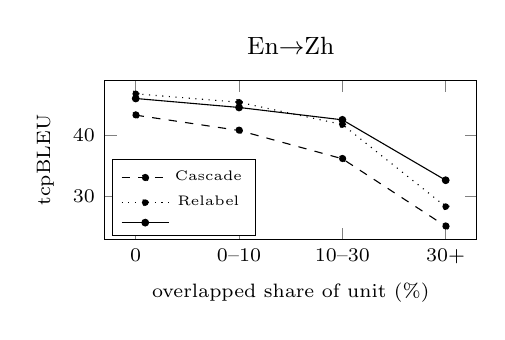
\begin{tikzpicture}\begin{axis}[width=0.52\columnwidth,height=3.6cm,xtick={0,1,2,3},
xticklabels={0,0--10,10--30,30+},xlabel={overlapped share of unit (\%)},ylabel={tcpBLEU},title={En$\rightarrow$Zh},
title style={font=\small},label style={font=\scriptsize},tick label style={font=\scriptsize},legend style={font=\tiny,at={(0.02,0.02)},anchor=south west}]
\addplot[dashed,mark=*,mark size=1.2pt] coordinates {(0,43.36) (1,40.84) (2,36.17) (3,25.04)}; \addlegendentry{Cascade}
\addplot[dotted,mark=*,mark size=1.2pt] coordinates {(0,46.88) (1,45.49) (2,41.82) (3,28.28)}; \addlegendentry{Relabel}
\addplot[solid,mark=*,mark size=1.2pt] coordinates {(0,46.11) (1,44.63) (2,42.59) (3,32.63)}; \addlegendentry{\sys{}}
\end{axis}\end{tikzpicture}
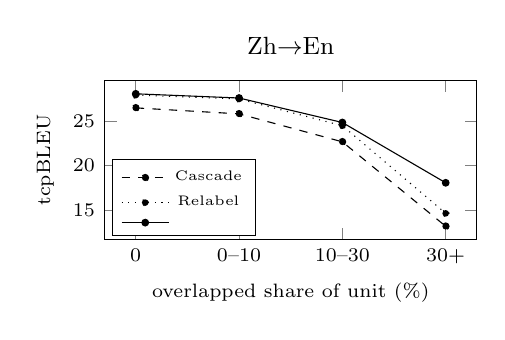
\begin{tikzpicture}\begin{axis}[width=0.52\columnwidth,height=3.6cm,xtick={0,1,2,3},
xticklabels={0,0--10,10--30,30+},xlabel={overlapped share of unit (\%)},ylabel={tcpBLEU},title={Zh$\rightarrow$En},
title style={font=\small},label style={font=\scriptsize},tick label style={font=\scriptsize},legend style={font=\tiny,at={(0.02,0.02)},anchor=south west}]
\addplot[dashed,mark=*,mark size=1.2pt] coordinates {(0,26.48) (1,25.81) (2,22.67) (3,13.19)}; \addlegendentry{Cascade}
\addplot[dotted,mark=*,mark size=1.2pt] coordinates {(0,27.91) (1,27.48) (2,24.48) (3,14.64)}; \addlegendentry{Relabel}
\addplot[solid,mark=*,mark size=1.2pt] coordinates {(0,28.06) (1,27.59) (2,24.84) (3,18.07)}; \addlegendentry{\sys{}}
\end{axis}\end{tikzpicture}
\caption{tcpBLEU by how much of a reference unit overlaps another speaker (reference windows, offline systems). The gap
between \sys{} and post-hoc relabelling opens where speakers overlap.}
\label{fig:overlap8}
\end{figure}


\paragraph{Labels or translation?} Relabelling \sys{}'s own output with the diarizer, keeping its text, separates the
two: on overlapped units its own labels score \num{v8:ov:en2zh:O2:ov} against
\num{v8:ov:en2zh:O2-relabel:ov} with diarizer labels (Zh$\rightarrow$En \num{v8:ov:zh2en:O2:ov} vs.\
\num{v8:ov:zh2en:O2-relabel:ov}), while with diarizer labels on both sides its text leads the speaker-blind model's by
\num{v8:ov:en2zh:O2-relabel:ov} vs.\ \num{v8:ov:en2zh:O2-nosd-relabel:ov}. Decoder-side speaker conditioning therefore mainly yields better
attributed segments under overlap: relabelling \sys{}'s own text costs \num{v8:ov:en2zh:O2:ov}$\rightarrow$\num{v8:ov:en2zh:O2-relabel:ov},
while its text with diarizer labels is only \num{v8:ov:en2zh:O2-relabel:ov} vs.\ \num{v8:ov:en2zh:O2-nosd-relabel:ov} for the
speaker-blind text; we do not claim that it translates overlapped speech better.

\paragraph{Short-turn fallback.} For every window, a cascade segment of at most 1.5\,s is added to \sys{}'s output
when no \sys{} segment of the same diarizer slot overlaps it within 0.5\,s and no nearby \sys{} text has chrF $\ge$50 with
it. On offline \sys{} this raises tcpBLEU in all three sets (Table~\ref{tab:overlap8}) and concurrent-speaker recall to
\num{v8:ov:en2zh:C2_O:cr} / \num{v8:ov:zh2en:C2_O:cr} / \num{v8:ov:ali:C2_O:cr}\%; on \sys{}-Simul it raises recall but
lowers tcpBLEU slightly, so by the criterion of the analysis plan it is adopted only for the offline model.

\paragraph{Latency.} Table~\ref{tab:lat8} queues the reads of a meeting on one decoder stream at the median single-stream
read time measured earlier (batch 1, two H200 cards, HuggingFace eager decoding). A wall-clock replay could only run beside another
job that held about \num{v8:b6:foreign_gib}\,GiB and most of the compute of every card,
with the Thinker spread over three cards at batch 1, so its real-time factor is an upper bound on the single-stream one.
On the one meeting completed (AliMeeting \num{v8:b6:ali_S2dl:meeting}, \sys{}-Simul) the median read took
\num{v8:b6:ali_S2dl:readp50}\,ms, \num{v8:b6:ali_S2dl:over}\% of the reads exceeded the 1\,s cadence, and the measured
real-time factor is \num{v8:b6:ali_S2dl:rtf}. By the rule of the analysis plan this is inconclusive, not a negative result:
contention only slows reads down, and an upper bound above 1 says nothing about the uncontended case. The remaining
replay runs were stopped, since further contended runs could not change that conclusion; two runs stopped part-way
(En$\rightarrow$Zh \sys{}-Simul, \num{v8:b6:en2zh_S2dl:done} of \num{v8:b6:en2zh_S2dl:of} windows; AliMeeting LocalAgreement,
\num{v8:b6:ali_O2_LA2:done} of \num{v8:b6:ali_O2_LA2:of}) are not used. The real-time factors of Table~\ref{tab:lat8} remain
estimates from the measured single-stream read time, not a replay.\ifWallclock{} A measured replay of the final systems is in Appendix~\ref{app:wallclock} (\sys{}'s Thinker does not keep up on AliMeeting).\fi{} LocalAgreement's reads take longer than the 1\,s read period, so queued it falls
behind without bound (per-speaker median \num{v8:lat:en2zh:O2_LA2:ps:p50}\,s). OpenSTBench-style start offset and
average delay of \sys{}-Simul (per-speaker channels, units spread uniformly over their block): \num{v8:lat:en2zh:S2dl:ps:start} and
\num{v8:lat:en2zh:S2dl:ps:atd}\,s in En$\rightarrow$Zh; these are not comparable with numbers reported on single-speaker
clips. Streams of more than 400 blocks (runaway repetition) were not synthesised: \num{v8:lat:ali:S2dl:ps:cens} on
AliMeeting, none elsewhere; counted as never heard, they leave the percentiles unchanged at the reported precision.

\paragraph{Fixed lag and seeds.} On an 8-meeting AMI subset (restricted for compute), fixed lag 2\,s on the
prefix-trained model scores \num{v8:sub:en2zh:lag2:all} tcpBLEU against \sys{}-Simul's \num{v8:sub:en2zh:on_S2dl:all} and
LocalAgreement's \num{v8:sub:en2zh:pla2:all} (En$\rightarrow$Zh; Zh$\rightarrow$En \num{v8:sub:zh2en:lag2:all} /
\num{v8:sub:zh2en:on_S2dl:all} / \num{v8:sub:zh2en:pla2:all}), but on overlapped units \num{v8:sub:en2zh:lag2:ov} vs.\
\num{v8:sub:en2zh:on_S2dl:ov} (\num{v8:sub:zh2en:lag2:ov} vs.\ \num{v8:sub:zh2en:on_S2dl:ov}), with a median text lag on
overlapped units of \num{v8:sub:en2zh:lag2:lagov} vs.\ \num{v8:sub:en2zh:on_S2dl:lagov}\,s. On the 10 AliMeeting subset
meetings (completed after the other runs, exploratory) fixed lag is ahead of \sys{}-Simul overall
and on overlapped units (\num{v8:sub:ali:lag2:all} / \num{v8:sub:ali:lag2:ov} vs.\ \num{v8:sub:ali:on_S2dl:all} /
\num{v8:sub:ali:on_S2dl:ov}; LocalAgreement \num{v8:sub:ali:pla2:all} / \num{v8:sub:ali:pla2:ov}), again at a longer lag on
overlapped units (\num{v8:sub:ali:lag2:lagov} vs.\ \num{v8:sub:ali:on_S2dl:lagov}\,s). Whole-meeting tcpBLEU of
\sys{}-Simul over training seeds: \num{v8:seed:en2zh:all} (En$\rightarrow$Zh, \num{v8:seed:en2zh:n} seeds; overlapped
\num{v8:seed:en2zh:ov}), \num{v8:seed:zh2en:all} (Zh$\rightarrow$En, \num{v8:seed:zh2en:n}), \num{v8:seed:ali:all}
(AliMeeting, \num{v8:seed:ali:n}).

\paragraph{Playback scheduling.} Table~\ref{tab:sched8} replays \sys{}-Simul's committed blocks under four single-channel
policies and the per-speaker layout. Captions for short overlapped interjections and skipping stale blocks bound the lag
of what is spoken, but on AliMeeting, where speakers overlap most, only \num{v8:b7:ali:d:cov}\% of the units are then
spoken.

\begin{table*}[t]
\centering\small
\begin{tabular}{lrrrrrrrrr}
\toprule
 & \multicolumn{3}{c}{En$\rightarrow$Zh} & \multicolumn{3}{c}{Zh$\rightarrow$En} & \multicolumn{3}{c}{AliMeeting} \\
\cmidrule(lr){2-4}\cmidrule(lr){5-7}\cmidrule(lr){8-10}
Playback & p50 & p90 & spoken & p50 & p90 & spoken & p50 & p90 & spoken \\
\midrule
one channel, as is & 142.4 & 772.6 & 100 & 26.4 & 313.0 & 100 & 604.6 & 2481.2 & 100 \\
short interjections as captions & 43.9 & 320.6 & 91 & 13.3 & 47.5 & 94 & 441.0 & 1630.3 & 93 \\
skip blocks $>$10\,s late & 9.7 & 11.8 & 80 & 9.8 & 13.1 & 82 & 10.8 & 17.2 & 35 \\
b + c & 9.1 & 11.6 & 80 & 9.4 & 12.9 & 82 & 10.8 & 17.4 & 35 \\
one channel per speaker, mixed & 7.4 & 12.2 & 100 & 8.2 & 15.1 & 100 & 23.2 & 314.1 & 100 \\
\bottomrule
\end{tabular}
\caption{Playback scheduling of \sys{}-Simul's whole-meeting output (reads queued; nothing re-synthesised, so the speech
of every played block is unchanged): listener completion lag (s) of the units played, and the share of units spoken
(\%; the rest are shown as captions). Policies fixed before any scheduling result.}
\label{tab:sched8}
\end{table*}


\paragraph{Voice prompts.} On 8 whole AMI En$\rightarrow$Zh meetings (3{,}318 output
streams), the Talker was run again with only the most recent 1\,s of a slot heard alone as its prompt instead of up to
8\,s, nothing else changed. The short prompt makes the voices less like the attributed speaker (WavLM SIM
\num{v8:b8:1s:sim} vs.\ \num{v8:b8:8s:sim}, meeting-bootstrap intervals \num{v8:b8:1s:simci} and \num{v8:b8:8s:simci}),
more often closer to another speaker of the window (\num{v8:b8:1s:conf} vs.\ \num{v8:b8:8s:conf}\%) and slightly less
intelligible (ASR-BLEU against the Talker's input \num{v8:b8:1s:asr} vs.\ \num{v8:b8:8s:asr}), so we keep 8\,s. At the
first commit \num{v8:b8:avail1}\% of the streams have 1\,s heard alone and \num{v8:b8:avail8}\% a full 8\,s. Holding a
slot's speech until 1\,s of it has been heard alone, instead of starting with the fallback prompt, would delay
\num{v8:b8:wait:streams}\% of the streams (\num{v8:b8:wait:blocks}\% of the blocks), but those by a median
\num{v8:b8:wait:p50}\,s (90th percentile \num{v8:b8:wait:p90}\,s): slots that rarely talk alone. Speaking at once is the
better default.

\paragraph{Threshold flips.} The causality check (Appendix~\ref{app:causal}) found \num{v8:b5:frames} distinct
80\,ms frames whose 0.5 activity decision differs between the prefix run and the dump. Rebuilding the online windows
with the prefix values changes \num{v8:b5:bound_same} window boundaries (none moves). The \num{v8:b5:windows} windows
holding a flipped frame were decoded again, each together with a copy using the original posteriors in the same batch:
\num{v8:b5:flip_same} are token-identical; an unchanged copy decoded in the same batch is identical in
\num{v8:b5:dup_same}. With so few windows the two cannot be told apart: the flips change outputs no more than
re-decoding does, but this check cannot show that they change nothing.

\paragraph{Full-coverage references.} The reference windows keep \num{v6:filt:en2zh:all:dur}\% of the En$\rightarrow$Zh
test speech. Every test utterance has a selected translation (Appendix~\ref{app:data}), so we also score the whole-meeting
runs on all \num{v8:full:en2zh:on_S2dl:units} non-hesitation units: \sys{}-Simul \num{v8:full:en2zh:on_S2dl:all}, LocalAgreement
on the offline model \num{v8:full:en2zh:on_O2_LA2:all}; overlapped units \num{v8:full:en2zh:on_S2dl:ov} vs.\
\num{v8:full:en2zh:on_O2_LA2:ov}. These are still machine translations.
